%\documentclass{article}
%%\def\pgfsysdriver{pgfsys-tex4ht.def}
%\usepackage[pdftex,active,tightpage]{preview}
%\usepackage{tikz}
%\begin{document}
%\begin{preview}
%%%%%%%%%%%%%%%%%%%%%%%%%%%%%%%%%
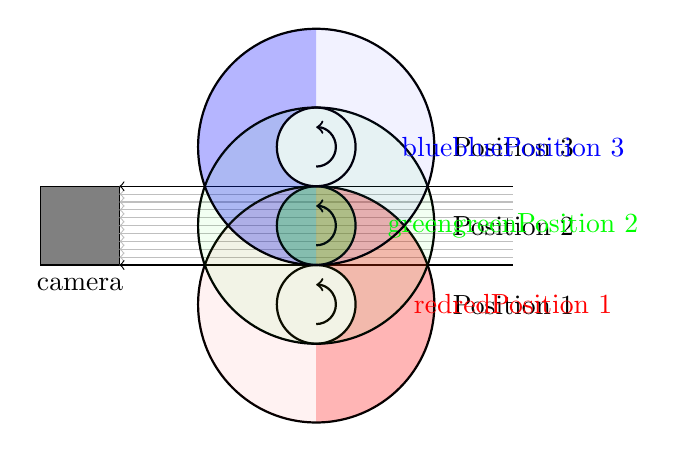
\begin{tikzpicture}
	\def\length{1}
	\def\beamlength{6}
	%grid
%	\draw[color=gray] (0,-3) grid (7,3);
	%camera
	\draw [fill=gray] (0,0) rectangle (\length,\length);
	\node at (.5*\length,-.25) {camera};
	% beam
	\foreach \x in {0,.1,...,1.1}
		\draw[gray!50,<-] (\length,\x) -- (\beamlength,\x);
	\foreach \x in {0,\length}
		\draw[<-] (\length,\x) -- (\beamlength,\x);
%	\node at (3.5*\length,\length+.25) {beam};
%%%%%	%colored samples
%%%%%	\foreach \y/\color/\position in {-.5/red/1,.5/green/2,1.5/blue/3}
%%%%%		{
%%%%%			\draw[thick,color=\color] (0.5*\beamlength+0.5*\length,\y) circle (1.5*\length) circle (.5*\length);
%%%%%			\draw[thick,->,color=\color] (0.5*\beamlength+0.5*\length,\y-.25*\length) arc (-90:90:0.25*\length);
%%%%%			\node[color=\color] at (\beamlength,\y) {Position \position};
%%%%%		}
	% filled samples
	\fill [color=red,nearly transparent]   (3.5,1) arc (90:-90:1.5*\length) -- ++(0,1) arc (-90:90:.5*\length);
	\fill [color=blue,nearly transparent]  (3.5,3) arc (90:270:1.5*\length) -- ++(0,1) arc (270:90:.5*\length);
	\fill [color=green,nearly transparent] (0.5*\beamlength+0.5*\length,.5) circle (0.5*\length);	
	\foreach \y/\position/\color in {-.5/1/red,.5/2/green,1.5/3/blue}
		{
			\draw[thick] (0.5*\beamlength+0.5*\length,\y) circle (1.5*\length) circle (.5*\length);
			\draw[thick,->] (0.5*\beamlength+0.5*\length,\y-.25*\length) arc (-90:90:0.25*\length);
			\fill [color=\color,ultra nearly transparent] (0.5*\beamlength+0.5*\length,\y) circle (1.5*\length);
			\node at (\beamlength+.005,\y-.005) {Position \position};
			\node [color=\color] at (\beamlength,\y) {Position \position};
		}
\end{tikzpicture}
%%%%%%%%%%%%%%%%%%%%%%%%%%%%%%%%%
%\end{preview}	
%\end{document}